\documentclass[11pt]{article}

\usepackage[final]{acl}
\usepackage{times}
\usepackage{latexsym}
\usepackage[T1]{fontenc}
\usepackage[utf8]{inputenc}
\usepackage{microtype}
\IfFileExists{inconsolata.sty}{\usepackage{inconsolata}}{}
\usepackage{graphicx}
\usepackage{booktabs}
\usepackage{xcolor}
\usepackage{amsmath}
\usepackage{multirow}
\usepackage{xurl}

% generated by src/analyze_annotations.py -- do not edit
\newcommand{\AlphaTrust}{0.66}
\newcommand{\AlphaSense}{0.47}
\newcommand{\AlphaTrustWithLLM}{0.58}
\newcommand{\LLMvsHumanQWK}{0.59}
\newcommand{\LLMvsHumanSenseKappa}{0.00}
\newcommand{\LLMSelfAlpha}{0.97}
\newcommand{\LLMvsHumanRho}{0.78}
\newcommand{\AUCHuman}{0.73}
\newcommand{\AUCLLM}{0.65}
\newcommand{\TrustCorrect}{3.66}
\newcommand{\TrustIncorrect}{2.88}
\newcommand{\LLMTrustCorrect}{4.12}
\newcommand{\LLMTrustIncorrect}{3.75}
\newcommand{\SenseCorrect}{71\%}
\newcommand{\SenseIncorrect}{47\%}
\newcommand{\RhoHumanRtwo}{0.25}
\newcommand{\RhoHumanConf}{0.90}
\newcommand{\MeanTrustHuman}{3.40}
\newcommand{\MeanTrustLLM}{4.00}
\newcommand{\LLMModel}{gpt-4o-mini}
\newcommand{\AlphaNoAuthor}{0.58}
\newcommand{\AUCNoAuthor}{0.69}
\newcommand{\AUCResidNoAuthor}{0.47}
\newcommand{\AUCAuthor}{0.76}
\newcommand{\AUCConf}{0.75}
\newcommand{\AUCResid}{0.51}
\newcommand{\PResid}{0.89}
\newcommand{\PTrustMW}{0.004}
\newcommand{\AUCLo}{0.60}
\newcommand{\AUCHi}{0.84}
\newcommand{\RhoLLMConf}{0.86}
\newcommand{\AUCLLMResid}{0.42}
\newcommand{\PairQWKRange}{0.57--0.79}

% generated by src/make_tables.py -- do not edit
\newcommand{\ReplRecallRange}{86.3--95.6}
\newcommand{\ReplRecallGap}{4.3}
\newcommand{\ReplTrustRange}{85.9--98.4}
\newcommand{\ReplTrustMAE}{2.0}
\newcommand{\ReplTrustAllMAE}{2.5}
\newcommand{\ReplTrustWithinFive}{7}
\newcommand{\IMDBLRRecall}{81.4}
\newcommand{\IMDBTreeRecall}{95.2}
\newcommand{\IMDBLimeTrustRange}{92.9--97.8}
\newcommand{\IMDBParzenTrustRange}{85.5--90.9}
\newcommand{\HeartLRRecall}{97.4}
\newcommand{\HeartTreeRecall}{66.4}
\newcommand{\HeartLimeTrustRange}{86.7--88.9}
\newcommand{\HeartParzenTrustRange}{91.5--94.9}

\newcommand{\repo}{\url{https://github.com/Sadhvika-Sunkara/lime-explainability-reproduction}}

\title{Reproducing and Extending LIME: Faithfulness and Trust of Local\\Explanations on New Text, Tabular and Human-Annotated Data}

\author{Sadhvika Sunkara \\
  Student ID 48768111 \\
  COMP8240 Applications of Data Science, Macquarie University \\
  \texttt{sadhvika.sunkara@students.mq.edu.au}}

\begin{document}
\maketitle

\begin{abstract}
We reproduce the two simulated-user experiments of \citet{ribeiro2016}, which introduced LIME, a model-agnostic method for explaining individual predictions. The authors' code is frozen at Python~2.7 and no longer installs, so we port it to Python~3 and re-run both experiments on the authors' original pre-processed Books and DVDs data. LIME's recall of the features a model truly uses is \ReplRecallRange{} (paper: 90.2--97.8), and its F1 for deciding whether a prediction can be trusted is \ReplTrustRange{} (paper: 91.8--96.7). LIME is the best of the four explainers in all 12 replicated settings (4 faithfulness, 8 trust), as the paper reports. We then apply the same protocols to two datasets the paper did not use, IMDB movie reviews and the UCI Heart Disease table, and build a new 60-item dataset of human and LLM-as-judge trust ratings of LIME explanations. LIME generalises well to new text. On tabular data its faithfulness to a decision tree falls to \HeartTreeRecall{}\%, and in the trust task a Parzen-window baseline matches or beats it. Three human raters agree well on trust (Krippendorff's $\alpha$\,=\,\AlphaTrust{}) and trust correct predictions more than wrong ones (AUC \AUCHuman{}). However, this is fully explained by the model confidence shown next to each prediction, and LIME's explanations add no detectable signal. An LLM judge (GPT-4o-mini) ranks items like the humans do ($\rho$\,=\,\LLMvsHumanRho{}) but is uniformly lenient: it accepted every explanation as sensible.
\end{abstract}

\section{Introduction}
Accurate classifiers are often opaque: a user cannot see why a particular prediction was made, and so cannot tell whether it rests on sensible evidence or on an artefact of the training data \citep{doshivelez2017}. \citet{ribeiro2016} proposed LIME (Local Interpretable Model-agnostic Explanations), which explains one prediction by fitting a sparse linear model to the black box's behaviour on perturbations of that input. The paper's central empirical claims are that LIME's explanations are \emph{faithful} to the model and \emph{useful for deciding whether to trust} a prediction.

This report (i) describes the paper and why it was chosen (\S\ref{sec:paper}) and its data (\S\ref{sec:data}); (ii) replicates its two simulated-user experiments with the original data and the authors' own code, ported to a modern stack (\S\ref{sec:repl}); (iii) builds new data: two existing datasets in a new text domain and a new modality, and a new human-annotated set of trust judgements (\S\ref{sec:newdata}); (iv) reports results on the new data, including an LLM-as-judge evaluation (\S\ref{sec:newres}); and (v) discusses ethics (\S\ref{sec:ethics}) and conclusions (\S\ref{sec:concl}). All code, results and the new annotations are public.\footnote{\repo}

%=====================================================================
\section{The Paper and Why We Chose It}
\label{sec:paper}
\paragraph{Method.} \citet{ribeiro2016}\footnote{\url{https://doi.org/10.1145/2939672.2939778}; preprint \url{https://arxiv.org/abs/1602.04938}} explain a prediction as follows. For an instance $x$, LIME draws $N$ perturbed samples $z$ around an interpretable representation $x'$ of $x$: for text, a binary bag of words, with perturbations that drop random subsets of the document's words. Each sample is weighted by a proximity kernel $\pi_x(z)$, and the explanation is
\begin{equation*}
\xi(x)=\operatorname*{argmin}_{g\in G}\;\mathcal{L}(f,g,\pi_x)+\Omega(g),
\end{equation*}
where $f$ is the black box, $G$ the class of sparse linear models, $\mathcal{L}$ the $\pi_x$-weighted squared loss and $\Omega$ caps the explanation at $K$ features. The authors select $K$ features along the LARS--lasso path and refit them by least squares (``K-LASSO''). The paper also proposes SP-LIME, a submodular procedure for choosing a small, non-redundant set of explanations to show a user. LIME later became the basis for SHAP \citep{lundberg2017} and Anchors \citep{ribeiro2018}.

\paragraph{Evaluation framework.} The paper evaluates explanations at three levels: simulated users with known ground truth, human users on simple tasks, and human users on real tasks. Its two quantitative simulated-user experiments, which are the targets of this reproduction, are:
\begin{itemize}\itemsep0pt
\item \textbf{Faithfulness (\S5.2).} Train classifiers whose truly used (``gold'') features are known: a sparse logistic regression (LR) and a decision tree (DT), each limited to ${\le}10$ features per prediction. Ask each explainer for $K{=}10$ features and measure the \emph{recall} of the gold features. LIME is reported at 90.2--97.8\% recall, against 17--21\% for a random explainer, 61--81\% for a Parzen-window approximation and 37--64\% for a greedy feature-removal procedure (paper Figs.~6--7).
\item \textbf{Trust in predictions (\S5.3).} Mark 25\% of the features as ``untrustworthy''. A prediction is truly untrustworthy if removing those features from the instance changes the prediction. A simulated user distrusts a prediction if, according to the explanation, removing the untrustworthy features would change it. The metric is F1 on the trustworthy class, averaged over 100 rounds, for LR, nearest-neighbour (NN), random forest (RF) and RBF-SVM classifiers. LIME scores 91.8--96.7 against at most 94.3 for Parzen, 58.1 for greedy and 14.8 for random (paper Table~1; reproduced in our Table~\ref{tab:trustrepl}).
\end{itemize}
The paper also reports human-subject studies, for example 27 graduate students judging a husky-vs-wolf classifier that had learned to detect snow. These require bespoke data and participants, and are not replication targets. Our new annotated dataset (\S\ref{sec:annot}) instead revisits their underlying question, whether people can use LIME to decide when to trust a prediction.

\paragraph{Justification.} \emph{Venue:} KDD is rated A* (the top tier, held continuously since CORE2008) in the ICORE2026 conference rankings \citep{icore2026}, and research.com places it 13th among all computer-science venues \citep{researchcom2026}. \emph{Impact:} Semantic Scholar records 23,899 citations \citep{semanticscholar2026}, making it one of the most cited papers in explainable AI. \emph{Reproducibility signals:} the experiment code is public \citep{limeexperiments}, the packaged library has about 12k GitHub stars \citep{limepackage}, the review datasets are public, and nothing needs a GPU. \emph{Room to extend:} the method is model-agnostic, so it applies to any new dataset; the paper's trust experiments use only synthetic ``untrustworthy'' features and few human raters---gaps our new data address.

%=====================================================================
\section{The Original Datasets}
\label{sec:data}
The quantitative experiments use two domains of the Multi-Domain Sentiment Dataset \citep{blitzer2007}:\footnote{\url{https://www.cs.jhu.edu/~mdredze/datasets/sentiment/}} Amazon reviews of \textbf{Books} and \textbf{DVDs}, with 1,000 positive (4--5 stars) and 1,000 negative (1--2 stars) reviews each. Following the authors' loader, each class is shuffled with seed~1 and split 80/20, giving 1,600 training and 400 test reviews per domain. Each review is a pseudo-XML record (Figure~\ref{fig:data}a) with product, rating, title, reviewer name, reviewer location, and free text. Only \texttt{review\_text} and the polarity are used. The authors' code reads not this raw text but the dataset's pre-processed release \texttt{processed\_acl}, in which each review is one line of \texttt{feature:count} pairs (unigrams and bigrams, e.g.\ \texttt{top\_secret:1 typhoon:1 \ldots{} \#label\#:positive}); their loader keeps the unigrams. We use the same file for the replication. On it the vocabularies are 19,502 (Books) and 19,046 (DVDs) word types, with about 85 distinct words per review. For a robustness check, and for comparability with IMDB, we also tokenise the raw review text (20,016 and 19,422 types, about 110 distinct words per review). The paper's other datasets were used only in its human-subject studies, which we do not replicate. (i)~The ``Christianity'' and ``Atheism'' documents of 20 Newsgroups \citep{lang1995} (1,079 training and 717 test posts in the standard split)\footnote{\url{http://qwone.com/~jason/20Newsgroups/}}, chosen because their e-mail headers contain features that do not generalise. (ii)~A \emph{religion} dataset the authors built from DMOZ and curated lists, with 819 Atheism and 819 Christianity web pages, used to test whether a classifier trained on 20 Newsgroups generalises; it was not released. (iii)~A husky-vs-wolf image set: a logistic-regression classifier trained on 20 hand-picked images, so that wolves always appear with snow, and evaluated on 60 further images by 27 graduate students. These images were not released either.

\begin{figure}[t]
\centering\scriptsize
\fbox{\parbox{0.95\columnwidth}{\ttfamily
\textbf{(a) Books, positive.review} (original data)\\
<review><asin>0743277724</asin> <product\_name>Pegasus Descending: A Dave Robicheaux Novel ...</product\_name> <rating>4.0</rating> <title>For lovers of Robicheaux</title> <reviewer>[redacted]</reviewer> <reviewer\_location>[redacted]</reviewer\_location> <review\_text>This book is for lovers of Robicheaux. His demons seem put to rest, redemption seems almost within his grasp - and yet the worst mayhem ever occurs within these pages. ...</review\_text></review>}}\\[3pt]
\fbox{\parbox{0.95\columnwidth}{\ttfamily
\textbf{(a$'$) processed\_acl/books/positive.review} (authors' input; one review per line)\\
holes:1 must:1 top\_secret:1 he:1 center:1 the\_pacific:1 the\_navy:1 a\_lot:1 this\_book:1 \ldots{} typhoon:1 pressure:1 strange:1 explored:1 \ldots{} \#label\#:positive}}\\[3pt]
\fbox{\parbox{0.95\columnwidth}{\ttfamily
\textbf{(b) IMDB} (new, existing): review,sentiment\\
"Probably my all-time favorite movie, a story of selflessness, sacrifice and dedication to a noble cause, but it's not preachy or boring. ...",positive}}\\[3pt]
\fbox{\parbox{0.95\columnwidth}{\ttfamily
\textbf{(c) processed.cleveland.data} (new, existing)\\ columns: age, sex, cp, trestbps, chol, fbs, restecg, thalach, exang, oldpeak, slope, ca, thal, num\\
63.0,1.0,1.0,145.0,233.0,1.0,2.0,\\\hspace*{1em}150.0,0.0,2.3,3.0,0.0,6.0,0\\
67.0,1.0,4.0,160.0,286.0,0.0,2.0,\\\hspace*{1em}108.0,1.0,1.5,2.0,3.0,3.0,2}}\\[3pt]
\fbox{\parbox{0.95\columnwidth}{\ttfamily
\textbf{(d) New annotated item H01} (constructed)\\
Patient: age 64; male; chest pain asymptomatic; BP 128; chol 263; max HR 105; exercise angina; ST depr.\ 0.2; slope flat; 1 vessel; thal reversible defect\\
Prediction: DISEASE (91\%)\\
LIME: thal=reversible defect $\rightarrow$ DISEASE (0.20); chest pain=asymptomatic $\rightarrow$ DISEASE (0.14); vessels=1 $\rightarrow$ DISEASE (0.13); exercise angina $\rightarrow$ DISEASE (0.09); sex=male $\rightarrow$ DISEASE (0.09)\\
Rater A/B/C: trust 1--5, makes sense Y/N \quad LLM: trust, makes sense, reason}}
\caption{Data snippets. Reviewer names and locations are redacted here although they are present in the public release (\S\ref{sec:ethics}).}
\label{fig:data}
\end{figure}

%=====================================================================
\section{Replication of the Original Work}
\label{sec:repl}
\paragraph{Environment.} The authors' code \citep{limeexperiments} pins Python~2.7, \texttt{numpy}~1.14, \texttt{scipy}~0.17 and \texttt{scikit-learn}~0.18. Those wheels do not exist for current Python versions, and the code uses Python~2 syntax and removed scikit-learn APIs (e.g.\ \texttt{sklearn.cross\_validation}). We therefore ported it to Python~3.13 with \texttt{scikit-learn}~1.9.1, \texttt{numpy}~2.5.3, \texttt{scipy}~1.18.1 and \texttt{lime}~0.2.0.1, on a 2-core Linux CPU machine. Earlier development ran on GitHub Codespaces and a Windows laptop. All versions are pinned in \texttt{requirements.txt}, \texttt{scripts/get\_data.py} downloads the data, and \texttt{run\_all.sh} re-runs every experiment. All replication scripts are in our public GitHub repository.\footnote{\repo{} (scripts in \texttt{src/}, raw results in \texttt{results/})}

\paragraph{What was ported, and how.} Our module \texttt{src/explainers.py} re-implements the four explainers from the authors' \texttt{explainers.py} and \texttt{parzen\_windows.py} with the same algorithms and hyperparameters: LIME with $N{=}15{,}000$ samples, kernel $\sqrt{\exp(-d^2/\rho^2)}$, $d=100\times$ cosine distance, $\rho{=}25$, and K-LASSO; Parzen fitted on 5-fold cross-validated predictions, using the authors' per-dataset bandwidths; greedy removal; and random selection. The scripts \texttt{run\_faithfulness.py} and \texttt{run\_trust.py} port \texttt{evaluate\_explanations.py} and \texttt{data\_trusting.py}, including their classifier settings (e.g.\ RF with 1,000 trees of depth 5, SVM with $C{=}10$, $\gamma{=}0.001$), seeds, the decision rules of the simulated users and the switched-sign F1 definition. Changes are limited to: (1)~Python~3 and current-API syntax; (2)~vectorised versions of the perturbation sampler, greedy search and Parzen gradient, each drawing from the same distribution as the original loops; and (3)~an exact closed-form RBF-SVM probability function for LIME's perturbations (\texttt{FastRBFSVC}; decision values match scikit-learn's to $10^{-11}$, probabilities to within libsvm's 0.005 coupling tolerance, verified in \texttt{tests/}). It is 6$\times$ faster, which made 15,000 samples per explanation affordable.

\paragraph{Input and deviations.} (a)~\emph{Input.} The replication uses the authors' exact input: the \texttt{processed\_acl} files, parsed with their own \texttt{get\_words} rule (regex \texttt{\textbackslash w*?:\textbackslash d}, bigrams dropped, each word repeated by its count) and vectorised as in their code (binary, no lower-casing). We repeat every experiment on the raw review text as a robustness check, since our new IMDB data is raw text as well. (b)~\emph{RF features.} The paper says its RF used averaged word2vec embeddings, but the released code's \texttt{random\_forest} option is a bag-of-words forest (the embedding variant needs an unreleased word2vec setup), so we use the code's version. (c)~\emph{Figure values.} Figs.~6--7 give recall values only as bar labels, which we transcribed and checked against the published figures. Table~1 values are printed in the paper.

\paragraph{An earlier, partial attempt.} Our project-update replication used the \texttt{lime} package's text explainer directly, with 80 Books test reviews, 1,000 samples, 10 rounds, LR only and a stop-word-filtered vocabulary. It reached a trust F1 of 97.5$\pm$0.9 for LIME (paper: 96.6), but it covered one of the paper's eight settings and none of its baselines. It also used a slightly different trust rule, comparing the local model with and without the untrustworthy words instead of comparing against the black box's own probability. The port described above replaces it and covers every setting of both experiments.

\subsection{Replicated results}
\begin{table*}[t]
\centering\small
\begin{tabular}{lcccccccc}
\toprule
 & \multicolumn{4}{c}{Books} & \multicolumn{4}{c}{DVDs} \\
\cmidrule(lr){2-5}\cmidrule(lr){6-9}
 & \multicolumn{2}{c}{Sparse LR} & \multicolumn{2}{c}{DT} & \multicolumn{2}{c}{Sparse LR} & \multicolumn{2}{c}{DT} \\
 & Ours & Paper & Ours & Paper & Ours & Paper & Ours & Paper \\
\midrule
Random & 17.1 & 17.4 & 14.6 & 20.6 & 13.9 & 19.2 & 13.1 & 17.4 \\
Parzen & 35.3 & 72.8 & 54.9 & 78.9 & 40.7 & 60.8 & 69.7 & 80.6 \\
Greedy & 45.5 & 64.3 & 28.0 & 37.0 & 51.2 & 63.4 & 38.1 & 47.6 \\
LIME & 86.3 & 92.1 & 89.7 & 97.0 & 88.3 & 90.2 & 95.6 & 97.8 \\
\midrule
Test acc. & 60.5 & -- & 63.0 & -- & 66.0 & -- & 64.8 & -- \\
\bottomrule
\end{tabular}

\caption{Replication of the faithfulness experiment (paper \S5.2, Figs.~6--7) on the authors' \texttt{processed\_acl} input: recall (\%) of the gold features by each explainer's top $K{=}10$, averaged over the 400 test reviews with a non-empty gold set. ``Paper'' values are the bar labels in the paper's figures. Test accuracy is that of the interpretable classifier, which the paper does not report.}
\label{tab:recallrepl}
\end{table*}

\begin{table*}[t]
\centering\small
\resizebox{\textwidth}{!}{\begin{tabular}{lcccccccc}
\toprule
 & \multicolumn{4}{c}{Books} & \multicolumn{4}{c}{DVDs} \\
\cmidrule(lr){2-5}\cmidrule(lr){6-9}
 & LR & NN & RF & SVM & LR & NN & RF & SVM \\
\midrule
Random & 14.7 {\scriptsize(14.6)} & 14.4 {\scriptsize(14.8)} & 14.7 {\scriptsize(14.7)} & 14.7 {\scriptsize(14.7)} & 14.9 {\scriptsize(14.2)} & 15.1 {\scriptsize(14.3)} & 14.8 {\scriptsize(14.5)} & 15.1 {\scriptsize(14.4)} \\
Parzen & 83.8 {\scriptsize(84.0)} & 90.4 {\scriptsize(87.6)} & 94.5 {\scriptsize(94.3)} & 89.5 {\scriptsize(92.3)} & 82.1 {\scriptsize(87.0)} & 80.4 {\scriptsize(81.7)} & 86.0 {\scriptsize(94.2)} & 82.4 {\scriptsize(87.3)} \\
Greedy & 54.5 {\scriptsize(53.7)} & 47.4 {\scriptsize(47.4)} & 48.3 {\scriptsize(45.0)} & 55.0 {\scriptsize(53.3)} & 53.6 {\scriptsize(52.4)} & 63.8 {\scriptsize(58.1)} & 60.4 {\scriptsize(46.6)} & 54.3 {\scriptsize(55.1)} \\
LIME & 96.5 {\scriptsize(96.6)} & 94.7 {\scriptsize(94.5)} & 98.3 {\scriptsize(96.2)} & 96.3 {\scriptsize(96.7)} & 96.7 {\scriptsize(96.6)} & 90.1 {\scriptsize(91.8)} & 98.6 {\scriptsize(96.1)} & 96.5 {\scriptsize(95.6)} \\
\midrule
Test acc. & 81.5 & 57.2 & 75.5 & 80.2 & 81.2 & 61.3 & 81.5 & 80.0 \\
Flipped & 11.3\% & 17.4\% & 9.7\% & 11.6\% & 11.4\% & 25.8\% & 10.7\% & 12.1\% \\
\bottomrule
\end{tabular}
}
\caption{Replication of the trust experiment (paper \S5.3, Table~1) on the authors' \texttt{processed\_acl} input: F1 (\%) of the trustworthy class, mean over 100 rounds with 25\% of the vocabulary untrustworthy. The paper's values are in brackets. ``Flipped'' is the share of test predictions the oracle marks untrustworthy. All differences between LIME and each baseline are significant ($t$-test, $p<10^{-4}$).}
\label{tab:trustrepl}
\end{table*}

\begin{table}[t]
\centering\small
\begin{tabular}{lcccc}
\toprule
 & \multicolumn{2}{c}{Trust F1 (8)} & \multicolumn{2}{c}{Recall (4)} \\
\cmidrule(lr){2-3}\cmidrule(lr){4-5}
Explainer & raw & acl & raw & acl \\
\midrule
Random & \MAERawTrustRandom & \MAEAclTrustRandom & \MAERawFaithRandom & \MAEAclFaithRandom \\
Parzen & \MAERawTrustParzen & \MAEAclTrustParzen & \MAERawFaithParzen & \MAEAclFaithParzen \\
Greedy & \MAERawTrustGreedy & \MAEAclTrustGreedy & \MAERawFaithGreedy & \MAEAclFaithGreedy \\
LIME & \MAERawTrustLime & \MAEAclTrustLime & \MAERawFaithLime & \MAEAclFaithLime \\
\bottomrule
\end{tabular}
\caption{Mean absolute difference from the paper (points) when the same code is run on our own tokenisation of the raw reviews (``raw'') and on the authors' pre-processed files (``acl''), over the 8 trust and 4 faithfulness settings.}
\label{tab:input}
\end{table}

\paragraph{Results.} Tables~\ref{tab:recallrepl} and~\ref{tab:trustrepl} give the replicated numbers next to the published ones. LIME is the best of the four explainers in all 12 settings (4 faithfulness, 8 trust), as the paper reports. The trust experiment replicates almost exactly. LIME's F1 is \ReplTrustRange{} against the paper's 91.8--96.7, a mean absolute difference of \ReplTrustMAE{} point, and all \ReplTrustWithinFive{} settings fall within the 5-point tolerance set in our proposal. Over all 32 explainer--setting pairs the mean difference is \ReplTrustAllMAE{} points, and several values are within 0.2 of the paper (e.g.\ Books LR: LIME 96.5 vs.\ 96.6, Parzen 83.8 vs.\ 84.0, Random 14.7 vs.\ 14.6). The ordering LIME $>$ Parzen $>$ Greedy $>$ Random holds in every trust setting, and per-round standard deviations are about 1 point (Table~\ref{tab:prf}). In the faithfulness experiment, LIME recovers \ReplRecallRange{}\% of the gold features against the paper's 90.2--97.8\%, \ReplRecallGap{} points lower on average. The paper's qualitative findings hold here too: Random is near chance, Greedy is much weaker on trees than on LR (and matches the paper's tree values, 37.1 vs.\ 37.0 on Books), and LIME leads every baseline.

\paragraph{The input matters more than the code.} Running the same code on our own tokenisation of the raw reviews (\S\ref{sec:data}) gives the same conclusions, but is consistently further from the paper (Table~\ref{tab:input}). The effect is small for LIME (\MAERawTrustLime{} vs.\ \MAEAclTrustLime{} points in trust), whose kernel only looks at the document's own words. It is large for Parzen's faithfulness (\MAERawFaithParzen{} vs.\ \MAEAclFaithParzen{} points). Parzen uses a squared-Euclidean kernel over the whole $\sim$20k-word vocabulary with bandwidths the authors tuned on their own files, so on raw text (about 110 instead of 85 distinct words per review) those bandwidths are wrong. Our bandwidth ablation on raw text (\texttt{src/ablation\_parzen\_sigma.py}) agrees: even the best $\sigma$, chosen on the test set, recovers only part of the gap (51--71\% recall), while the authors' input brings Parzen to within \MAEAclFaithParzen{} points of the paper on average.

\paragraph{Remaining differences.} \emph{(1) LIME's recall for the Books sparse LR} is 85.1 against 92.1 (95\% CI $\pm$2.5). With $C{=}0.03$ the model keeps only 6 non-zero words (test accuracy 58\%), so each document has about two gold words and one miss costs 50\%. Which 6 words are selected may depend on solver details that changed between scikit-learn 0.18 and 1.9. We consider this the most likely cause, but could not test it without the original stack. \emph{(2) The decision trees are unpruned (depth 49--53)}, as in the released code, although the paper says no prediction uses more than 10 features and its figure files are named \texttt{shallow\_tree}. We tested a depth-10 tree (\texttt{--tree-max-depth 10}). It changes LIME's recall by only about a point, in opposite directions (Books \BooksDeepTreeLime{}$\rightarrow$\BooksShallowTreeLime{}, DVDs \DvdDeepTreeLime{}$\rightarrow$\DvdShallowTreeLime{}), and it moves Greedy far from the paper (Books 60.2 vs.\ 37.0, DVDs 58.9 vs.\ 47.6). So the paper most likely used the unpruned tree, and tree depth is ruled out as a cause. \emph{(3) Parzen's trust F1 on DVDs} is 1--8 points low, most of all with RF (86.0 vs.\ 94.2). The authors' DVD bandwidths are small ($\sigma{=}0.5$--$0.75$, against 0.5--7 for Books), so the Parzen estimate rests on very few neighbours and is sensitive to small differences in the data; we did not test this further. \emph{(4) RF} uses bag-of-words features, as in the released code, instead of the embedding forest described in the paper. This is the most likely reason its Greedy values differ most (60.4 vs.\ 46.6 on DVDs).


%=====================================================================
\section{Construction of New Data}
\label{sec:newdata}
We use two existing datasets that the paper did not, chosen to vary one property each relative to the original data, and construct one new annotated dataset.

\paragraph{IMDB (new text domain).} The Large Movie Review Dataset \citep{maas2011}\footnote{\url{https://ai.stanford.edu/~amaas/data/sentiment/}} contains 50,000 movie reviews, balanced between positive and negative, distributed as a single CSV of \texttt{review,sentiment} pairs (Figure~\ref{fig:data}b). Its reviews are longer than the product reviews (231 vs.\ 170 tokens per review on average). To keep everything else equal to the replication, we draw a balanced random sample of 1,000 positive and 1,000 negative reviews (seed 1), remove HTML line breaks, and apply exactly the Books/DVDs pipeline: 80/20 split, binary bag of words, same classifiers, same explainers, $K{=}10$. Parzen bandwidths, which the authors tuned per dataset, are chosen by their own criterion (least disagreement with the classifier's cross-validated predictions).

\paragraph{UCI Heart Disease (new modality).} The processed Cleveland subset of the UCI Heart Disease data \citep{janosi1988,detrano1989}\footnote{\url{https://archive.ics.uci.edu/dataset/45/heart+disease}, CC BY 4.0} has 303 patients and 13 clinical attributes (Figure~\ref{fig:data}c): 5 continuous (age, resting blood pressure, cholesterol, maximum heart rate, ST depression) and 8 categorical (sex, chest-pain type, fasting sugar, resting ECG, exercise angina, ST slope, vessels coloured, thallium test). We drop the 6 records with missing \texttt{ca}/\texttt{thal} (297 remain) and binarise the target (0 = no disease, 1--4 = disease; 46\% positive). Tabular data exercises LIME's other perturbation mode, which samples features from training statistics and discretises continuous features into quartiles, and the paper does not evaluate it quantitatively. Adapting the protocols required three decisions: (i)~``removing'' a feature means resetting it to its training median (continuous) or mode (categorical), which the oracle, greedy and Parzen all use; (ii)~$K{=}5$ of 13 features, since $K{=}10$ would make recall nearly trivial, and the trust experiment marks 3 of 13 features (25\%) as untrustworthy; and (iii)~a 60-patient test set is too small to score, so every patient is explained by a model trained on the other four folds of a stratified 5-fold split (cross-fitting). LIME here is the official \texttt{lime} package's tabular explainer with $N{=}15{,}000$ samples.

\subsection{New human-annotated trust dataset}
\label{sec:annot}
To test the paper's motivating claim with real people rather than simulated users, we built an \emph{explanation-trust} dataset of 60 Heart Disease predictions. The model is the random forest from our project update (300 trees, depth 6), with cross-fitted accuracy 84.8\% (252/297). We sampled 20 incorrect and 40 correct predictions (seed 1) and shuffled them. Errors are over-sampled relative to their 15\% base rate, so that there is enough signal to test whether raters can spot predictions that should not be trusted. Sixty items kept each rater's task to about 25 minutes, which mattered for unpaid volunteers. The cost is precision: the AUCs in \S\ref{sec:humanres} have 95\% bootstrap intervals about $\pm$0.12 wide, enough to tell the raters from chance but not to detect small effects. Each item shows the patient's full record in plain language, the predicted class and confidence, and LIME's top-5 explanation, worded as ``fact $\rightarrow$ towards DISEASE / NO DISEASE (weight)'' (Figure~\ref{fig:data}d). Raters answer \textbf{Q1} ``How much do you trust this prediction?'' (1 = strongly distrust \ldots{} 5 = strongly trust) and \textbf{Q2} ``Does the explanation make sense given the patient record?'' (Yes/No). They never see the true label. The sheet (\texttt{annotation/annotation\_sheet.xlsx}) includes a participant-information and consent page, a worked example row and input validation.

\paragraph{Annotators and agreement.} Three annotators (the author and two classmates, none with clinical training) rated all 60 items independently. This is a limitation: annotator~A is the author, who designed the study and knew its aims, so her ratings may not be independent. She did not have the answer key (true labels and correctness) when rating, but that does not remove the bias. We therefore release every rater's ratings separately and repeat the main analysis without her (\S\ref{sec:humanres}). Unpaid volunteers stand in for the paper's paid Mechanical Turk workers. We measure agreement with Krippendorff's $\alpha$ \citep{krippendorff2011}, ordinal for Q1 and nominal for Q2, because it handles ordinal data and missing ratings; our implementation reproduces the reference values in that paper. We also report pairwise quadratic-weighted Cohen's $\kappa$ \citep{cohen1968}.

\paragraph{LLM-as-judge.} The same 60 items, with the same instructions and questions, were given to an LLM (\LLMModel{}, temperature 0, JSON output, three independent repeats; \texttt{src/llm\_judge.py}), which also never saw the true label. The judge plays the role of an additional, scalable annotator \citep{zheng2023}. We check it in two ways: \emph{agreement} with the human consensus (quadratic-weighted $\kappa$ against the median human rating; $\kappa$ against the Q2 majority), and \emph{validity}, i.e.\ whether its trust ratings separate correct from incorrect predictions as well as human ratings do (ROC AUC).

%=====================================================================
\section{Results on New Data}
\label{sec:newres}
\begin{table}[t]
\centering\small
\resizebox{\columnwidth}{!}{\begin{tabular}{lcccc}
\toprule
 & \multicolumn{2}{c}{IMDB (text, $K{=}10$)} & \multicolumn{2}{c}{Heart (tabular, $K{=}5$)} \\
\cmidrule(lr){2-3}\cmidrule(lr){4-5}
 & Sparse LR & DT & Sparse LR & DT \\
\midrule
Random & 11.8 & 11.0 & 38.2 & 39.0 \\
Parzen & 45.7 & 17.9 & 40.7 & 45.3 \\
Greedy & 49.6 & 36.2 & 28.2 & 28.2 \\
LIME & 81.4 & 95.2 & 97.4 & 66.4 \\
\midrule
Mean $|$gold$|$ & 3.3 & 1.6 & 4.8 & 4.4 \\
\bottomrule
\end{tabular}
}
\caption{Faithfulness on new data: recall (\%) of gold features. Same protocol as Table~\ref{tab:recallrepl}. Heart uses $K{=}5$ of 13 features, so Random's expected recall is about 38\%.}
\label{tab:recallnew}
\end{table}

\begin{table*}[t]
\centering\small
\resizebox{0.8\textwidth}{!}{\begin{tabular}{lcccccccc}
\toprule
 & \multicolumn{4}{c}{IMDB} & \multicolumn{4}{c}{Heart} \\
\cmidrule(lr){2-5}\cmidrule(lr){6-9}
 & LR & NN & RF & SVM & LR & NN & RF & SVM \\
\midrule
Random & 12.8 & 12.6 & 12.9 & 12.8 & 32.3 & 31.3 & 32.0 & 32.1 \\
Parzen & 85.7 & 85.5 & 90.9 & 90.5 & 93.3 & 91.5 & 94.0 & 94.9 \\
Greedy & 48.0 & 45.9 & 45.4 & 48.8 & 66.9 & 60.2 & 65.0 & 60.5 \\
LIME & 95.3 & 92.9 & 97.8 & 95.2 & 87.7 & 86.7 & 88.9 & 87.4 \\
\midrule
Test acc. & 82.5 & 57.8 & 79.0 & 81.5 & 83.8 & 82.5 & 83.8 & 83.5 \\
Flipped & 12.1\% & 25.2\% & 12.3\% & 12.1\% & 9.9\% & 14.6\% & 9.1\% & 9.0\% \\
\bottomrule
\end{tabular}
}
\caption{Trust on new data: F1 (\%) of the trustworthy class, same protocol as Table~\ref{tab:trustrepl}. Heart: 3 of 13 features untrustworthy, $K{=}5$, 297 patients via 5-fold cross-fitting. All LIME--baseline differences are significant ($p<10^{-4}$). On Heart, Parzen is significantly \emph{better} than LIME.}
\label{tab:trustnew}
\end{table*}

\begin{figure*}[t]
\centering
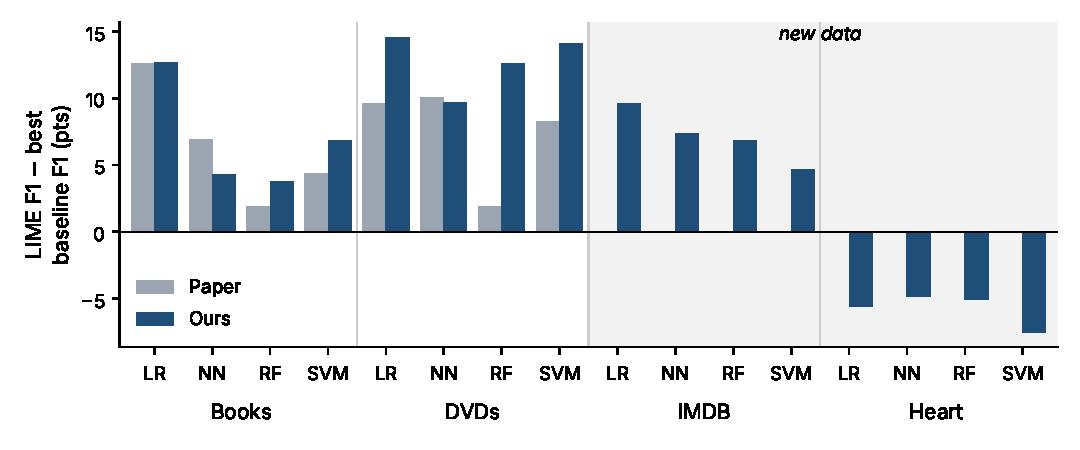
\includegraphics[width=0.85\textwidth]{generated/fig_trust_margin.pdf}
\caption{LIME's margin over the best of the three baselines in the trust experiment (F1 points). Grey bars are the paper's Table~1, dark bars are ours. The margin is preserved in every replicated setting and on IMDB, and turns negative on tabular Heart data.}
\label{fig:margin}
\end{figure*}

\subsection{Simulated-user experiments}
\paragraph{New text domain (IMDB).} LIME generalises to movie reviews. In the trust experiment its F1 is \IMDBLimeTrustRange{} (Table~\ref{tab:trustnew}), which is within the range of the replication (\ReplTrustRange{}), and the method ordering is unchanged. Parzen (\IMDBParzenTrustRange{}) and Greedy behave as on Books/DVDs. For faithfulness (Table~\ref{tab:recallnew}), LIME recovers \IMDBTreeRecall{}\% of the tree's gold words, close to Books and DVDs (94.1 and 96.5). For the sparse LR it recovers \IMDBLRRecall{}\%, below Books and DVDs (85.1 and 90.9). IMDB reviews have about 147 distinct words, against 85 in the authors' Books/DVDs files, so each document has more candidate words competing for the same $K{=}10$ slots, and the sampler drops a smaller fraction of the relevant words in each perturbation. Even so, LIME's recall is 32 points above the next-best explainer.

\paragraph{New modality (Heart Disease).} The tabular results diverge from the paper's conclusions in two ways. \emph{Faithfulness:} LIME recovers \HeartLRRecall{}\% of the sparse LR's gold features but only \HeartTreeRecall{}\% of the decision tree's, against 94.1--96.5\% on the three text datasets. The tabular explainer discretises continuous features into training-set quartiles and perturbs by resampling bins, so a split in the tree at, say, \texttt{oldpeak}\,${\le}\,0.7$ can fall inside a quartile. Perturbations then rarely cross the threshold and the feature looks locally irrelevant. On text there is no such mismatch, because removing a word is exactly the operation a word-presence split tests. \emph{Trust:} Parzen (\HeartParzenTrustRange{}) significantly outperforms LIME (\HeartLimeTrustRange{}) for all four classifiers (Figure~\ref{fig:margin}). Table~\ref{tab:prf} shows why: LIME's precision stays high (92--96\%) but its recall falls to 82--84\%, so it distrusts too many trustworthy predictions. LIME's interpretable features for tabular data mean ``the patient is in bin $b$'', and the trust rule removes a feature by subtracting its weight, which is equivalent to moving the patient \emph{out of} that bin. The oracle instead resets the feature to its training median or mode, and for 45\% of (patient, feature) pairs that leaves the patient in the same bin (37\% exactly unchanged, e.g.\ \emph{sex = male} is also the mode). LIME therefore predicts a change where none happens. Our Parzen adaptation measures the change towards exactly that baseline, so part of its advantage comes from the evaluation design. That is itself the finding: LIME's tabular explanations describe deviation from the training distribution, not from a particular reference value, and a user who reads ``removing this feature'' literally will be misled. The paper's text-only evaluation could not reveal this.

\paragraph{Against the replication.} The new data agrees with the replication on text and disagrees on tables. On IMDB, LIME is again the best explainer in every setting, its trust F1 (\IMDBLimeTrustRange{}) lies inside the replicated range (\ReplTrustRange{}), and its recall of the tree's features (\IMDBTreeRecall{}\%) matches Books and DVDs. On Heart Disease, two of the replication's conclusions fail: LIME's recall of the tree's features falls to \HeartTreeRecall{}\%, and Parzen, never better than LIME in any replicated setting, beats it in all four trust settings.

\subsection{Human and LLM trust judgements}
\label{sec:humanres}
% Numbers come from report/generated/annotation_macros.tex (src/analyze_annotations.py).
\paragraph{Agreement between people.} All three annotators completed all 60 items (one Q2 answer was left blank). Inter-annotator agreement on trust is Krippendorff's $\alpha$\,=\,\AlphaTrust{} (ordinal), and pairwise quadratic-weighted $\kappa$ ranges over \PairQWKRange{}, i.e.\ moderate to substantial agreement. Agreement on whether an explanation ``makes sense'' is lower ($\alpha$\,=\,\AlphaSense{}, nominal), so judging the medical plausibility of a reason is harder for non-experts than giving an overall trust rating. Annotator C was the most sceptical, and the mean trust over all ratings is \MeanTrustHuman{} on the 1--5 scale.

\paragraph{Do explanations help people spot wrong predictions?} Correct predictions received a mean human trust of \TrustCorrect{}, and incorrect ones \TrustIncorrect{} (Mann--Whitney $p$\,=\,\PTrustMW{}). Averaged trust separates correct from incorrect predictions with ROC AUC \AUCHuman{} (95\% bootstrap CI \AUCLo{}--\AUCHi{}; 0.5 is chance), and explanations were judged to make sense for \SenseCorrect{} of correct but only \SenseIncorrect{} of incorrect predictions. On the face of it this supports the paper's claim. However, human trust correlates almost perfectly with the model confidence printed next to each prediction (Spearman $\rho$\,=\,\RhoHumanConf{}), and confidence \emph{alone} separates correct from incorrect predictions just as well (AUC \AUCConf{}). Once confidence is regressed out, the remaining variation in human trust carries no signal about correctness (AUC \AUCResid{}, $p$\,=\,\PResid{}), and trust correlates only weakly with LIME's local fidelity ($\rho$\,=\,\RhoHumanRtwo{}). Our raters could tell good predictions from bad, but we find no evidence that LIME's explanations contributed beyond the confidence score. Because every item showed both, the design cannot rule out a smaller effect; an explanation-versus-no-explanation condition would be needed to measure it (\S\ref{sec:concl}).

\paragraph{LLM-as-judge.} The judge (\LLMModel{}, three repeats) is almost perfectly self-consistent ($\alpha$\,=\,\LLMSelfAlpha{}), and it ranks items much as people do: Spearman $\rho$\,=\,\LLMvsHumanRho{} with the mean human rating, and quadratic-weighted $\kappa$\,=\,\LLMvsHumanQWK{} with the human median. That is within the range of agreement between the humans themselves (\PairQWKRange{}). As a rater, however, it is systematically lenient. Its mean trust is \MeanTrustLLM{} against \MeanTrustHuman{} for humans, it never gave a rating below 3 (humans gave 1--2 in 18\% of ratings), and it answered ``Yes, the explanation makes sense'' for all 180 judgements, against 63\% for humans. Agreement with the human Q2 majority is therefore $\kappa$\,=\,\LLMvsHumanSenseKappa{} by construction, and adding the judge as a fourth rater \emph{lowers} the group's $\alpha$ from \AlphaTrust{} to \AlphaTrustWithLLM{}. Its trust separates correct from incorrect predictions less well than the humans' (AUC \AUCLLM{} vs.\ \AUCHuman{}; mean \LLMTrustCorrect{} vs.\ \LLMTrustIncorrect{}). Like the humans, it mostly follows the displayed confidence ($\rho$\,=\,\RhoLLMConf{}), and beyond confidence it carries no signal (AUC \AUCLLMResid{}). Its stated reasons are generic (e.g.\ ``the explanation aligns with the patient's clinical attributes that are known risk factors''). This confirms the risk anticipated in our proposal: an LLM judge accepts fluent, plausible-sounding explanations rather than checking them. It is a cheap, reproducible proxy for the \emph{ranking} of human trust, but not a substitute for human judgement of whether an explanation is sound.


\paragraph{How this evaluation differs from the replication.} The simulated-user experiments define an untrustworthy prediction as one that depends on randomly designated ``untrustworthy'' features, and the simulated user applies a fixed rule to the explanation. In the annotation study, ground truth is whether the prediction is actually correct, and the users are people (or an LLM) who bring their own prior beliefs about heart disease. The paper's human studies were closer to this but used text classifiers and Mechanical Turk workers. Ours applies the question to tabular clinical data, the setting in which the simulated results above suggest LIME is least reliable.


%=====================================================================
\section{Ethical Considerations}
\label{sec:ethics}
\paragraph{In the original paper.} (1)~\emph{Human participants.} The trust and model-selection studies used Amazon Mechanical Turk workers and the husky/wolf study used 27 graduate students. The paper says nothing about ethics approval, consent, or how much crowdworkers were paid, all of which are now normally reported. (2)~\emph{Personal data in public corpora.} The review data carries reviewer names and locations (Figure~\ref{fig:data}a), and 20 Newsgroups carries e-mail headers, author names and signatures. The paper uses these headers to show that a classifier can rely on spurious identity cues, but redistributing and mining the corpora still exposes people who never agreed to research use. (3)~\emph{Deliberately misleading models.} The husky/wolf classifier was trained to be wrong in order to test whether people notice. That is a legitimate design, but it shows explanations being used to manage trust, and a persuasive explanation can raise trust in a bad model as easily as lower it. Later work shows that LIME can be gamed to hide a biased model \citep{slack2020} and is unstable under small input changes \citep{alvarezmelis2018}.

\paragraph{If we published on our new data.} We consider the principles of the \emph{Australian Code for the Responsible Conduct of Research} \citep{nhmrc2018} and the \emph{National Statement on Ethical Conduct in Human Research} \citep{nhmrc2025} that apply.
\begin{itemize}\itemsep1pt
\item \textbf{Human participants (respect, fairness).} Our three raters are human participants. The task carries no foreseeable risk beyond minor inconvenience, which places it at the lower end of the National Statement's risk continuum, but publishing it would still require review under Macquarie's human-research ethics process before data collection. As a classroom exercise, we used an information sheet, opt-in consent (typing an annotator code), the right to withdraw ratings until submission, and pseudonymous codes, with only aggregate results reported. Recruiting classmates creates a mild peer-pressure dynamic, so participation was voluntary and unrewarded, and no one was asked twice.
\item \textbf{Health data (respect, accountability).} The Cleveland records are de-identified and released under CC BY 4.0, but they are clinical records collected in 1988 for diagnostic research, under consent norms we cannot inspect. We use them only for a methodological question, do not attempt re-identification, and present every prediction as a study artefact, never as medical advice. The model and its explanations are not clinically validated. The sheet says so, and so does this paper.
\item \textbf{Bias that explanations expose.} 68\% of the Cleveland patients are male, and their disease rate is 56\% against 26\% for women. Sex appears among LIME's top five reasons in 32 of our 60 annotated explanations (Figure~\ref{fig:data}d). An explanation that makes a demographic attribute look like legitimate evidence can lend it false authority. A faithful explanation of a biased model is still an explanation of a biased model, and a publication should report subgroup performance.
\item \textbf{Third-party data and licences (recognition, honesty).} IMDB and the Blitzer reviews are research releases without explicit redistribution licences, so our repository ships download scripts rather than copies. The CC BY 4.0 Heart data is included with attribution. We redact reviewer identities in figures.
\item \textbf{LLM-as-judge (transparency, accountability).} Sending items to a commercial API is acceptable under Macquarie's AI policy \citep{mqaipolicy} only because they hold de-identified public data and no rater information. We name the model and settings and release prompts and outputs. LLM judgements are reported as a separate, validated signal and are never mixed into the human ratings.
\item \textbf{Open science and honesty (transparency, rigour).} Code, environment, results, the annotation sheet, the anonymised ratings and the answer key are public. Deviations from the original protocol are listed in \S\ref{sec:repl} and not hidden, and every reported number is regenerated from the result files.
\end{itemize}


%=====================================================================
\section{Conclusions and Reflections}
\label{sec:concl}
\paragraph{Replication.} Both simulated-user experiments of \citet{ribeiro2016} replicate. With the authors' algorithms and settings ported to Python~3, LIME is the best of the four explainers in all 16 settings. Its trust F1 is within \ReplTrustMAE{} points of the published values on average, and its faithfulness recall is \ReplRecallGap{} points lower on average. The largest discrepancy, the Parzen baseline's faithfulness, is partly explained by bandwidths tuned to the authors' unavailable pre-tokenised features (our ablation) and otherwise by that input change. The paper is therefore reproducible in substance but not exactly: exact reproduction would need the frozen Python~2 stack and the \texttt{processed\_acl} files, and it is this dependency, not the method, that has decayed.

\paragraph{Generalisation.} On a new text domain (IMDB), every conclusion carries over. On a new modality (tabular clinical data), two do not: LIME is much less faithful to decision trees (\HeartTreeRecall{}\% recall), and a simple Parzen baseline beats it at telling trustworthy from untrustworthy predictions. We trace the second result to what LIME's tabular explanations mean, deviation from the training distribution rather than from a reference value. For tabular data, a practitioner should therefore read LIME weights as ``relative to a typical patient'', not ``what would happen if this value were removed''. With real people the picture is more cautious: raters agreed well and trusted correct predictions more, but the model's displayed confidence explains all of that discrimination, so in our data the explanations themselves did not measurably help people decide when to trust a prediction. An LLM judge reproduced the humans' ranking but accepted every explanation, so it cannot yet replace human evaluation of explanation quality.

\paragraph{Reflections.} (1)~\emph{Reproducibility decays through the environment more than through the paper.} The method and evaluation were described clearly enough to re-implement, but the pinned 2016 stack no longer installs and one input format is no longer linked. Version-pinned containers and released processed data would have avoided both problems. (2)~\emph{Protocols do not transfer between modalities for free.} The paper's notion of ``removing'' a feature is clear for words but not for a blood-pressure reading. Our choice (reset to the median or mode) is defensible, but it directly affects which explainer looks best, which suggests that explanation benchmarks should state their removal semantics explicitly. (3)~\emph{Annotation is harder than it looks.} Raters without clinical training must judge both the model and the medicine, and moderate agreement is expected. In hindsight, a larger set of items with simpler, non-medical content would separate ``trust in the explanation'' from ``trust in one's own medical intuition'' more cleanly. A design where each rater sees the same item both with and without an explanation would isolate the explanation's effect. (4)~\emph{Our earlier pipeline gave a more flattering number.} The project-update run reported a trust F1 of 97.5 on one setting with a simplified trust rule. The faithful port gives 95.5. Small protocol simplifications can bias a replication towards ``success'', which is why we kept the original rules even where they look odd (e.g.\ explaining the true rather than the predicted label in \S5.2).


\paragraph{Use of AI tools.} I designed this project in my proposal: the choice of paper, the replication targets and tolerance, the two new datasets, the human trust study and the LLM-as-judge comparison. I ran the exploratory experiments (\texttt{earlier\_attempts/}), including the Heart Disease model the annotators rated, recruited and briefed the annotators and rated as annotator~A, ran the LLM judge, obtained the authors' original data and verified the paper's figure values. I used Claude (Anthropic), as permitted for this assessment, to port the authors' code to Python~3, write and run the experiment and analysis scripts, build the annotation sheet and draft the report from the results. I reviewed and checked every section, and I take responsibility for every claim, number and reference.

\bibliography{references}

\appendix
\section{Experimental details}
\label{app:details}
\begin{table}[h]
\centering\small
\begin{tabular}{p{0.32\columnwidth}p{0.58\columnwidth}}
\toprule
Setting & Value \\
\midrule
Text features & binary bag of words, lower-cased, scikit-learn tokeniser, no stop-word removal \\
Split & 1,000 pos.\ + 1,000 neg.; per class shuffled (seed 1), 80/20 $\rightarrow$ 1,600 / 400 \\
Sparse LR (\S5.2) & L1, liblinear; $C$ lowered from 0.1 in steps of 0.01 until every training doc uses ${\le}10$ features ($C{=}0.03$ for all three text sets) \\
DT (\S5.2) & unpruned CART, seed 1 (text); depth 5 (Heart) \\
\S5.3 classifiers & LR (L2, default $C$); $k$NN ($k{=}5$); RF (1,000 trees, depth 5); SVM (RBF, $C{=}10$, $\gamma{=}0.001$, Platt) \\
LIME (text) & $N{=}15{,}000$; kernel $\sqrt{\exp(-d^2/25^2)}$, $d = 100\times$cosine; K-LASSO; $K{=}10$ \\
LIME (Heart) & \texttt{lime} 0.2.0.1 tabular, quartile discretisation, $N{=}15{,}000$, $K{=}5$ \\
Parzen $\sigma$ & paper values for Books/DVDs; for IMDB/Heart chosen by leave-one-out disagreement with 5-fold CV predictions \\
Trust rounds & 100; 25\% of features untrustworthy (Heart: 3 of 13) \\
Heart removal & feature $\rightarrow$ training median (continuous) / mode (categorical) \\
Heart evaluation & stratified 5-fold cross-fitting, all 297 patients explained once \\
\bottomrule
\end{tabular}
\caption{Hyperparameters. Everything not listed follows \citet{limeexperiments}.}
\label{tab:hyper}
\end{table}

\begin{table}[h]
\centering\small
\begin{tabular}{llccc}
\toprule
Data & Clf. & P & R & F1 ($\pm$sd) \\
\midrule
Books & LR & 94.7 & 98.4 & 96.5 $\pm$ 0.8 \\
 & NN & 92.5 & 97.0 & 94.7 $\pm$ 1.1 \\
 & RF & 97.6 & 99.1 & 98.3 $\pm$ 0.6 \\
 & SVM & 94.8 & 97.9 & 96.3 $\pm$ 0.8 \\
\midrule
DVDs & LR & 95.0 & 98.4 & 96.7 $\pm$ 0.8 \\
 & NN & 86.8 & 93.7 & 90.1 $\pm$ 1.5 \\
 & RF & 98.1 & 99.2 & 98.6 $\pm$ 0.5 \\
 & SVM & 95.2 & 97.8 & 96.5 $\pm$ 0.7 \\
\midrule
IMDB & LR & 92.6 & 98.3 & 95.3 $\pm$ 1.2 \\
 & NN & 89.6 & 96.5 & 92.9 $\pm$ 2.1 \\
 & RF & 96.7 & 98.9 & 97.8 $\pm$ 0.7 \\
 & SVM & 92.6 & 98.0 & 95.2 $\pm$ 1.0 \\
\midrule
Heart & LR & 95.6 & 81.5 & 87.7 $\pm$ 8.1 \\
 & NN & 91.8 & 82.4 & 86.7 $\pm$ 6.1 \\
 & RF & 95.1 & 83.8 & 88.9 $\pm$ 8.1 \\
 & SVM & 94.8 & 81.5 & 87.4 $\pm$ 7.0 \\
\bottomrule
\end{tabular}

\caption{LIME's precision and recall for the trustworthy class (\S5.3 protocol), mean over 100 rounds. Recall is consistently high on text. On Heart the lower recall means LIME flags too many trustworthy predictions as untrustworthy.}
\label{tab:prf}
\end{table}

\paragraph{Annotator instructions (verbatim summary).} ``You are asked to rate 60 predictions made by a machine-learning model that estimates whether a patient has heart disease, each shown with an automatic explanation (LIME) \ldots{} The explanation lists up to 5 facts about the patient and whether each pushed the model towards DISEASE or NO DISEASE; a larger weight means a stronger push. Q1 How much do you trust this prediction? (1 = strongly distrust, 2 = distrust, 3 = unsure, 4 = trust, 5 = strongly trust). Q2 Does the explanation make sense given the patient record? (Yes/No).'' The LLM judge receives the same text as its system prompt (\texttt{src/llm\_judge.py}).


\end{document}
